A major challenge in transferring the knowledge from the source is to design a strategy to combine the source knowledge with the knowledge from the target task. In this section, we propose propose a combination strategy that using linear argumentation to combine the source and target knowledge. An important advantage of this strategy is that we can adjust the impact of the knowledge comes from the source model more flexibly by just modifying the value of its coefficient (called transfer parameter). As long as the source knowledge hurts the transfer model, we can reduce its impact to avoid negative transfer.

\hl{we generally assume that we can't access the source data}

\subsection{$\mathcal{D}$-relationship between the hypothesis and the distribution}
\hl{Intuitively}, when transferring the knowledge from another task, the performance of the model for the target task is greatly determined by the relationship of these two tasks. Here we use the $\mathcal{H}$-divergence to measure the relationship of two different tasks. $\mathcal{H}$-divergence can be defined as follow:
\begin{defi} \label{single:hdivergence}
	(from Kifer et al. \cite{kifer2004detecting}) Given a domain $\mathcal{X}$ with two probability distributions, let $\mathcal{H}$ be a hypothesis class on $\mathcal{X}$ and denote by $I(h)$ the set for which $h \in \mathcal{H}$ is the characteristic function where $x\in I(h) \leftrightarrow h(x)=1$. The $\mathcal{H}$-divergence between these two probability distribution $D$ and $D'$ is 
	\begin{equation*}
	{d_{\mathcal{H}}}\left( {D,D'} \right) = 2\mathop {\sup }\limits_{h \in {\mathcal{H}}} \left| {{{\Pr }_D}\left[ {I(h)} \right] - {{\Pr }_{D'}}\left[ {I(h)} \right]} \right|
	\end{equation*}
\end{defi}
When $d_{\mathcal{H}}\left( {D,D'} \right)$ is small. it means for any $(x,y) \in D$ and $(x',y') \in D'$, if $y=y'$, there exists a hypothesis $h$ such that the difference between $h(x)$ and $h(x')$ can be small with a high probability. Otherwise, they are unrelated. From its definition we can see that $\mathcal{H}$-divergence is a metric to measure the dissimilarity of two distributions. The more similar two distributions are, the smaller $\mathcal{H}$-divergence is. Ben et al. \cite{ben2010theory} show that the performance of the target model is affected by the $\mathcal{H}$-divergence of the probability distributions of the two tasks. Specifically, the smaller $\mathcal{H}$-divergence is, the more benefit the transfer model can get from the source task.

Suppose $D$ and $D'$ are two distributions for the binary classification problem with class labels $\{1,-1\}$ and there is a binary hypothesis $h'$ that is consistent with $D'$, i.e. for any $(x',y') \in D'$, $h'(x')=y'$.
If $D$ and $D'$ are related, according to Definition \ref{single:hdivergence}, for any example $(x,y) \in D$, we would expect a high probability for $\Pr_{(x,y)\sim D}(h'(x)=y)$. Here, we call the hypothesis $h'$ and distribution $D$ are positive related. On the other hand, as $D'$ is a distribution for binary classification problem, we can use $-h'$ to denote the complement of the hypothesis $h'$. If $-h'$ is consistent with $D'$, we should expect a high probability for $\Pr_{(x,y)\sim D}(h'(x)=-y)$. Here we call the hypothesis $h'$ and distribution $D$ are negative related. We use $d_{h'\sim D'}(D)$ to denote the $\mathcal{D}$-relationship of the hypothesis $h'$ and the distribution $D$. The $\mathcal{D}$-relationship of a hypothesis $h'$ and a distribution $D$ is defined as follow:
\begin{defi}\label{single:drelation}
Let $D$ and $D'$ be two distributions for the binary classification problem $\{1,-1\}$. Given a hypothesis $h'$ consistent with $D'$ and , the $\mathcal{D}$-relationship of the hypothesis $h'$ and the distribution $D$ can be written as:
\begin{equation*}
%%{d_{h'\sim D'}}(D) = \max \left(\underset{\text{Positive Sum}}{\left| {\sum\limits_{(x,1) \in D} {h'(x)} } \right|} + \underset{\text{Negative Sum}}{\left| {\sum\limits_{(x, - 1) \in D} {h'(x)} } \right|}\right)
{d_{h'\sim D'}}(D) = \min \left(\underset{\text{Positive term}}{\Pr_{(x,y)\sim D}(h'(x)=y)} , \underset{\text{Negative term}} {\Pr_{(x,y)\sim D}(h'(x)=-y)}\right)
\end{equation*}
\end{defi}
Here we call the two terms $ {\sum_{(x,1) \in D} {h'(x)} } $ and ${\sum_{(x, - 1) \in D} {h'(x)} } $ positive and negative terms respectively.
As we discussed above, when $h'$ and $D$ are positive related, we should expect most positive and negative examples in $D$ be classified as positive and negative in hypothesis $h'$. Therefore, ${d_{h'\sim D'}}(D)$ equals $\Pr_{(x,y)\sim D}(h'(x)=y)$. When they are negative related,  ${d_{h'\sim D'}}(D)$ equals $\Pr_{(x,y)\sim D}(h'(x)=-y)$. Therefore, when $h'$ and $D$ are related, the $\mathcal{D}$-relationship should be large. When $h'$ and $D$ are unrelated, the output of $h'$ should be more random for both positive and negative examples. Therefore, both positive and negative terms are closed to 0.5 and the ${d_{h'\sim D'}}(D)$ should be closed to 0.5 as well. Obviously, $\mathcal{D}$-relationship describes the agreement of the hypothesis $h'$ and the distribution $D$. In a binary classification scenario, $h'$ and $D$ are related if $h'$ is highly agree with $D$ (positive related) or disagree with $D$ (negative related). If $\mathcal{D}$-relationship is closed to 0.5, $h'$ and $D$ are unrelated. Similarly, we can get a conclusion based on the conclusion of \cite{ben2010theory} that the smaller $\mathcal{D}$-relationship is, the less benefit a transfer model can get from the source model(s).

\subsection{Leverage the Source Knowledge with Data Arguementation}
Then our self-defined category learning problem can be described as follow: Given a task $T$ to distinguish whether an example is from one certain category $C$ from a domain $\mathcal{X} \times \mathcal{Y}$ with $D$ probability distribution over $\mathcal{X}$, $\mathcal{X}$ is the input feature and $\mathcal{Y}$ is the label set $\{1,-1\}$. We use an examples with label 1 to denote the positive example (i.e. belongs to the category) and an example with label -1 to denote the negative example (i.e. not belong to this category). There is another group of binary source models $F'=\{f'_{1},...,f'{n}\}$ trained from another independent task $S$ on another domain $\mathcal{X'} \times \mathcal{Y'}$ with $D'$ probability distribution over $\mathcal{X'}$. The $F'$ and $D$ are related. Given a small training set $T_{train}=\{(x,y)\} \subset \mathcal{X}\times \mathcal{Y}$, $\mathcal{X}$, our target task is to learn a classification model $f: \mathcal{X} \rightarrow \mathcal{X}$ from $T_{train}$ incorporating with $F'=\{f'_{1},...,f'{k}\}$ so that $f$ can perform well on an independent testing set $T_{test}=\{(x,y)\} \subset \mathcal{X} \times \mathcal{Y}$.

Here, let's set the both source and target model $f$ and $F'$ in the hypothesis space of function $\mathcal{H}$ which equals to space of all the linear models of the form. 
\begin{equation}
f(x)=w^Tx+b
\end{equation}
%where $\phi(x)$ is a feature mapping that maps the input space into a another high or even possible infinite dimensional space.
\begin{figure}
	\centering
	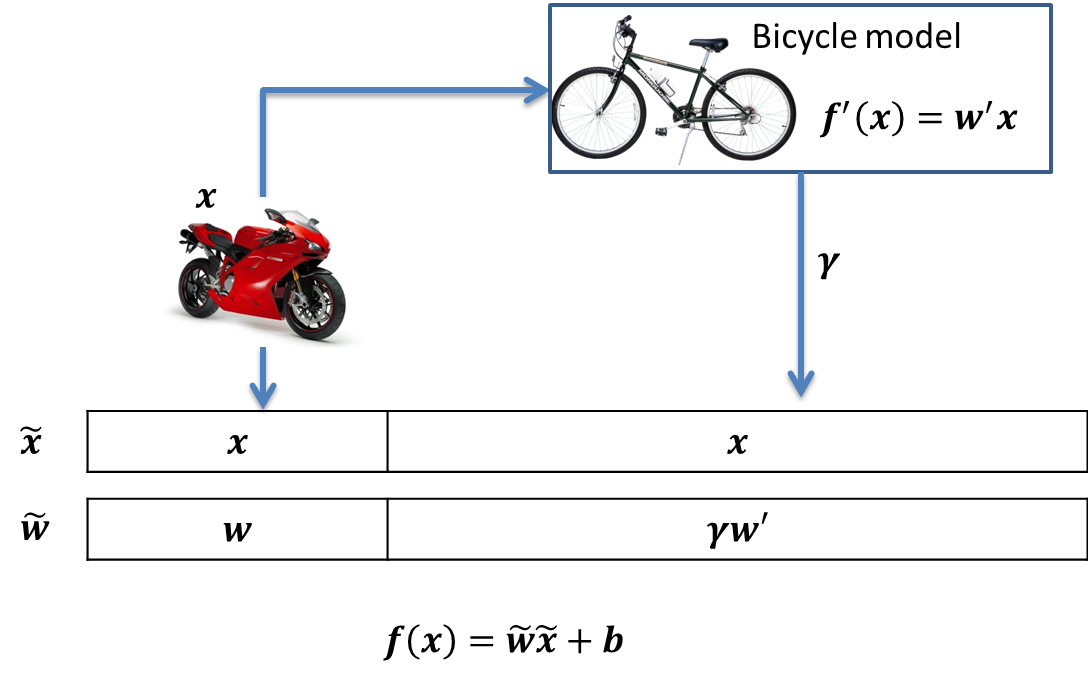
\includegraphics[scale=.7]{transfer/fig/argumentation.png}
	\caption{A graphical representation of linear argumentation. The score from the source model can be considered as an auxiliary feature and the transfer parameter controls the value of the auxiliary feature. For linear classifiers, it can be considered as a linear combination of the decision from the source model and target data (see \eqref{eq:single:linear}).}\label{fig:single:arg}
\end{figure}

To leverage the knowledge from the source models $F'$, we consider to use the decision scores from the source model as the auxiliary information and use the auxiliary information to adjust the decision for our transfer model. 
By introducing the auxiliary information from the source models, we can have several advantages especially when we use linear model such as SVM.

The first advantage is simplicity. Given an example $x$ and the source models $F'$, we can simply add the decision scores of each $f_i'(x)$ from $F'$ to the target model to affect its decision. This process can be written as:

\begin{equation}\label{eq:single:linear}
\begin{aligned}
f(x) = & w^Tx+b+\sum_{i=1}^{k}\gamma_i f_i'(x) \\
\text{st.} \qquad & f_i'(x) = w_i'^Tx
\end{aligned}
\end{equation}

Here $\gamma=\{\gamma_1,....,\gamma_k\}$ is a hyper-parameter to control the amount of the knowledge transferred from each of the source model $f_i'$. This process is equivalent to the data argumentation approach where the scores of the source model is used as the auxiliary feature (see Figure \ref{fig:single:arg}). 
By introducing the auxiliary information from the source model, we expect to reduce the bias from the target training set and get an improvement from the auxiliary feature. With this data argumentation, the transfer learning problem becomes a traditional machine learning problem. The transfer model can be determined as long as we get the hyperplane $w$
 
Another advantage is flexibility. As the decision scores from the source model are used as the auxiliary knowledge. By using the transfer parameters to control the amount of the knowledge from each source model, the model for the target task is more adaptive to different situations. If the knowledge from the source model is related, we should increase its impact, i.e. , otherwise, its impact should be decreased. 

In the previous work \cite{kuzborskij2013n} \cite{tommasi2014learning}, according to the definition of $\mathcal{H}$-divergence, they consider that there are only two relationships between the target task and a source model: related or unrelated. When they are related, the transfer parameter should be set to positive and 0 otherwise. In our work, according to Definition \ref{single:drelation}, there could be 3 different relationships between the target task and a specific source model: unrelated, positive related and negative related. 

For a multi-class scenario, our goal is to use a linear system to distinguish different categories with One-VS-All strategy. For each category, we should build a binary classification model and assign the label according to $sign\left[f(x)\right]$. According to Eq. \eqref{eq:single:linear}, for any example $x$, the decision score of our binary model consist of two parts: a score learned from our target task which is the term of $w^Tx+b$ and the knowledge from the source models, i.e. $\sum_{i}\gamma_i f_i'(x)$. In order to
The transfer parameters should be set as follow:
\begin{itemize}
	\item When the source model and the target task are not related, according to Definition \ref{single:drelation}, the expectation of the decision score from the source model is closed to be 0.5 and it can't provide much useful information for the target task. Therefore, the auxiliary feature from this source model is considered to be redundant. Thus, to eliminate its affect, the transfer parameter should be set closed to 0. As a result, the impact of the decision of the source model is minimized and the target model is less likely to suffer from negative transfer. In the extreme case where the transfer parameter is set 0, no auxiliary information is introduced to adjust the bias in the target task and therefore, we can guarantee that, at least, negative transfer won't happen.
	\item When the source and target tasks are negative related, i.e. the expected decision score for positive examples in target task is negative and for positive 
\end{itemize}

\begin{figure}
	\centering
	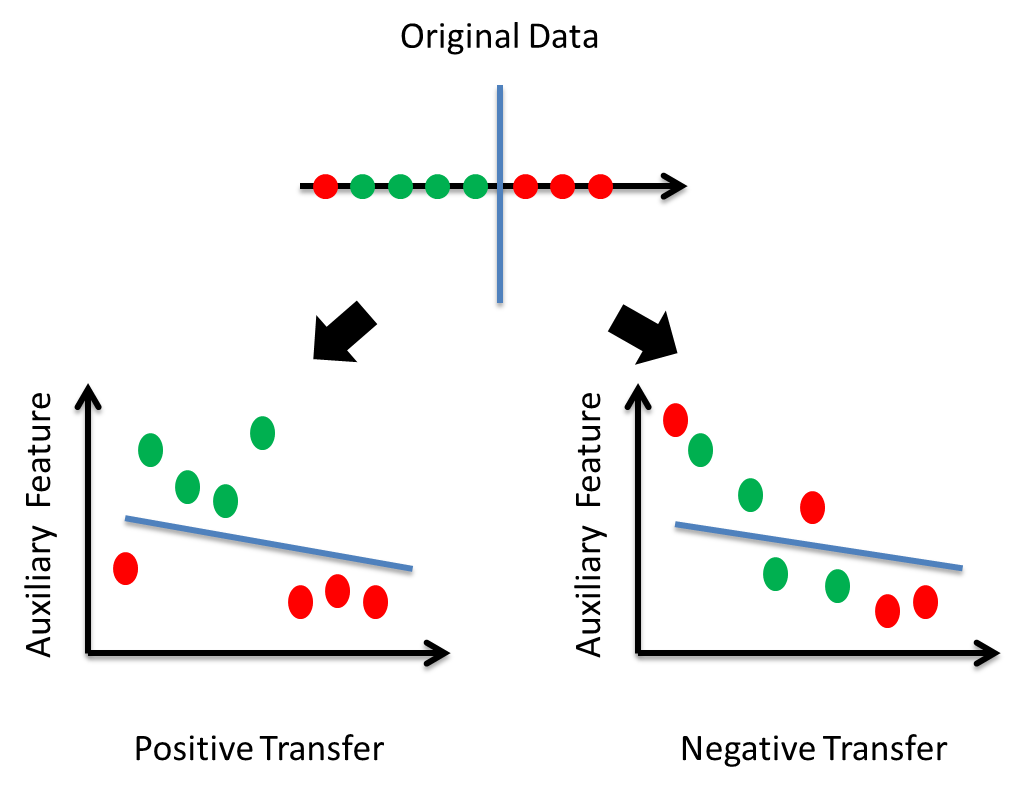
\includegraphics[scale=.7]{transfer/fig/dataarg.png}
	\caption{Suppose the original data is one dimensional and we use the blue line to denote the optimal decision surfce of a linear model (the upper figure). By adding an related auxiliary feature, we can improve the performacne of the classifier (the bottom-left figure) while unrelated one can decrease the performance and lead to negative transfer (the bottom-right figure). }\label{fig:single:dataarg}
\end{figure}

Therefore, let $\tilde{x} = (x,f_1'(x),...,f'_k(x))$ and $\tilde{w} = (w,\gamma_1,....,\gamma_k)$.
With the LS-SVM setting, our transfer problem can be solved by solving the following optimization problem with argument data:
\begin{equation}\label{eq:single:reg}
	\begin{aligned}
	\min \qquad& L_{LSSVM}(\tilde{w}) = \frac{1}{2}{\left\| \tilde{w} \right\|^2} + \frac{C}{2}\sum\limits_{i = 1}^l {{e_i ^2}}\\
	\text{s.t.}\qquad& \tilde{w} = (w,\gamma_1,....,\gamma_k)\\
	&{y_i} = \tilde{w} {\tilde{x_i}} + b + {e _i} \quad   \text{for} \quad i \in \left\{ {1,2,...,l} \right\}\\
	\end{aligned}
\end{equation}
Here, we can treat $\gamma$ and $w$ as a whole parameter $\tilde w$ and solve the problem \eqref{eq:single:reg} directly with the method described in subsection \ref{sec:single:lssvm} to obtain the values of them. However, this would case serious problem if the dimension of $w$ is much larger than the dimension of $\gamma$. In this situation, 

 
When we consider the transfer parameter $\gamma$ as a hyperparameter that can be determined by certain prior knowledge. To regularize  $\left\|\tilde{w}\right\|^2$ is equivalent to regularize $\left\|\tilde{w}-\gamma w'\right\|^2$. Therefore, function \eqref{eq:single:reg} can be represented as:
\begin{equation}\label{eq:single:formreg}
\begin{aligned}
\min \qquad& L_{\gamma}(w) = \frac{1}{2}{\left\| {w}-\sum\limits_{i}^{n}\gamma_i w'_i \right\|^2} + \frac{C}{2}\sum\limits_{i = 1}^l {{e_i ^2}}\\
\text{s.t.}\qquad& {y_i} = {w} {{x_i}} + b + {e _i} \quad   \text{for} \quad i \in \left\{ {1,2,...,l} \right\}\\
\end{aligned}
\end{equation}

To solve the problem \eqref{eq:single:formreg}, we first introduce some important notations used in the rest of this chapter in Table \ref{tab:single:notation}. We use any letter with apostrophe to denote the information from the source data, e.g. if $f(x)$ denotes the model for the target task, $f'(x)$ denotes the model for the source one.

% Table generated by Excel2LaTeX from sheet 'Sheet1'
\begin{table}
	\centering
	\caption{\hl{Notations used in this chapter}}
	\begin{tabular}{|c|L{14cm}|}
		\hline
		$f'(x)$ & binary model for source task \\
		\hline
		$f(x)$  & binary model for target task \\
		\hline
		$\phi(x)$ &  function mapping the input sample into a high dimensional feature space. \\ \hline
		%    $K(x,x)$ & kernel matrix with  $\phi(x_i) \cdot\phi(x_j)$ corresponding to its element $(i,j)$\\ \hline
		$X$     & instance matrix with each row representing one instance \\\hline
		$\boldsymbol{W} $    & (N+1)-column hyperplane matrix for target task. Each column represents one hyperplane of a binary model \\\hline
		$\boldsymbol{W'}$    & hyperplane matrix for the source task \\\hline
		$\boldsymbol{a'} $   & the Lagrangian multiplier matrix for source problem. Each column represents a set of Lagrangian multiplier for a binary SVM model \\\hline
		$\boldsymbol{a} $    & the Lagrangian multiplier matrix for target problem \\
		\hline
		$\boldsymbol{b'},\boldsymbol{b}$  & the bias vector for source and target task \\
		\hline
		$\boldsymbol{a_i}$ & $i_{th}$ column of matrix $\boldsymbol{a}$ \\ \hline
		%    $d_\gamma$ &  diagonal matrix with$\left[ {{\gamma _1},...,{\gamma _N}} \right]$ in its main diagonal\\\hline
		$\boldsymbol{\beta}$ & row vector $\left[ {{\beta _1},...,{\beta _N}} \right]$ to control the prior knowledge for the new category\\ \hline
		$\varepsilon_{ny_i}$&loss parameter. $\varepsilon _{n{y_i}}=1$ if $n=y_i$ and 0 otherwise\\ \hline
		$\psi$, $\psi^{-1}$ & $\psi$ is the modified kernel matrix for solving binary LS-SVM and $\psi^{-1}$ is the inverse matrix of $\psi$\\ \hline
	\end{tabular}%
	\label{tab:single:notation}%
\end{table}%

The primal Lagrangian for this optimization problem \ref{eq:single:formreg} given the unconstrained minimization problem can be written as: 
\begin{equation}
	{L_\gamma }\left( {w,b,\alpha ,e} \right) = \frac{1}{2}{\left\| {w - \sum\limits_{i}^{n}\gamma_i w'_i} \right\|^2} + \frac{C}{2}\sum\limits_{i = 1}^l {{e _i}^2}  - \sum\limits_{i = 1}^l {{\alpha _i}\left\{ {w{x_i} + b + {e_i} - {y_i}} \right\}} 
\end{equation}
The optimal solution can be found by satisfying the following condition:
\begin{eqnarray}\label{eq:single:lssvm-deriv}
\begin{aligned}
\frac{{\partial L}}{{\partial w}} = 0 &\to w = \sum\limits_{i}^{n}\gamma_i w'_i + \sum\limits_i^l {{\alpha _i}{x_i}} \\
\frac{{\partial L}}{{\partial b}} = 0 &\to \sum\limits_i^l {{\alpha _i} = 0} \\
\frac{{\partial L}}{{\partial e_i}} = 0 &\to C{e_i} = {\alpha _i} \qquad i = 1,...,l\\
\frac{{\partial L}}{{\partial {\alpha _i}}} = 0 &\to {y_i} = {w} {{x_i}} + b + {e _i}\qquad i = 1,...,l\\
\end{aligned}
\end{eqnarray}

Let $X=\left[x_1,x_2,...,x_l\right]$ and $Y=[y_1,y_2,...,y_l]$, Eq \eqref{eq:single:lssvm-deriv} can be written in the following compact format:

\begin{equation}\label{eq:single:matrixsolve}
	\left[\begin{array}{cc}
	XX^T+\frac{\mathbf{I}}{C}&\mathbf{1}\\
	\mathbf{1}^T&0
	\end{array}\right]\left[\begin{array}{c} \mathbf{\alpha}\\b
	\end{array}\right] = \left[\begin{array}{c} Y\\0
	\end{array}\right]
\end{equation} 
where $\mathbf{1}$ is a column  vector whose elements are 1. 

In real applications, when we have $n$ single source categories and their corresponding source model $f'_1(x),f'_2(x),...,f_n(x)$, their loss function can be represented as:

\begin{equation}\label{eq:single:unionreg}
\begin{aligned}
\min \qquad& L_{\gamma}(w_1,w_2,...,w_n) = \frac{1}{2}\sum\limits_{i = 1}^n{\left\| {w_i}-\gamma_i w_i' \right\|^2} + \frac{C}{2}\sum\limits_{i = 1}^n\sum\limits_{j = 1}^l {{e_{ij} ^2}}\\
\text{s.t.}\qquad& {y_{ij}} = {w_i} {{x_i}} + b_i + {e _{ij}} \quad   \text{for} \quad i \in \left\{ {1,2,...,l}  \right\}, j \in {1,2,...,n}\\
\end{aligned}
\end{equation}
Let $\mathbf{W} = [w_1,w_2,...,w_n]$, $\mathbf{W'} = [w'_1,w'_2,...,w'_n]$ and $D(\gamma)$ be the diagonal matrix $diag(\gamma_1,\gamma_2,...,\gamma_n)$. The corresponding solution for problem \eqref{eq:single:unionreg} is:

\begin{equation}\label{eq:single:multisolu}
\left[\begin{array}{cc}
XX^T+\frac{\mathbf{I}}{C}&\mathbf{1}\\
\mathbf{1}^T&0
\end{array}\right]\left[\begin{array}{c} \mathbf{\alpha}\\b
\end{array}\right]+\left[\begin{array}{c}
D(\gamma)X(W')^T\\0
\end{array}\right] = \left[\begin{array}{c} Y\\0
\end{array}\right]
\end{equation} 
Here $Y = [y_{ij}|i=1,..,l; j=1,...,n]$ is the encoded label matrix where for each example $(x_i,y_i)$:
\begin{equation}\label{eq:single:labelmatrix}
	y_{ij}=
	\begin{cases}
	1 & \text{if } y_i=j\\
	-1 &\text{otherwise}
	\end{cases}
\end{equation}
We can see that Eq. \eqref{eq:single:unionreg} can be solved by directly once the transfer parameters $\gamma=\{\gamma_i|i=1,...,n\}$ is determined.

To summarize this section, we propose a strategy which uses linear combination to combine the knowledge of the source model and the knowledge from the target dataset. We show that this linear combination strategy can be considered as a data argumentation approach and thus, the transfer learning problem becomes a traditional machine learning problem. Moreover, we show that by setting different values of the transfer parameters, we can control the amount of the knowledge from the source model effectively. In the next section, we show that we can estimate the cross-validation error of the LS-SVM in a closed form.


